\documentclass[11pt]{article}

\usepackage[margin=1in]{geometry}
\usepackage{graphicx}
\usepackage{booktabs}
\usepackage{array}
\usepackage{tikz}
\usetikzlibrary{arrows.meta, positioning, shapes.geometric, fit, backgrounds}
\usepackage{xcolor}
\usepackage{hyperref}
\usepackage{caption}
\usepackage{float}
\usepackage{amsmath}
\usepackage{listings}
\usepackage{enumitem}

\hypersetup{colorlinks=true, linkcolor=blue, urlcolor=blue, citecolor=blue}

\definecolor{boxblue}{RGB}{221,235,247}
\definecolor{boxgreen}{RGB}{226,239,218}
\definecolor{boxorange}{RGB}{252,228,214}
\definecolor{boxgray}{RGB}{242,242,242}

\title{\vspace{-1.5cm}\textbf{Hex-Recognition VLM}\\[4pt]
\large A Small Vision Model for Hexadecimal-to-Decimal Conversion:\\
Dataset Generation, Architecture Ablation, Generalization, RL Design, and Deployment}
\author{Sajjad Shahali}
\date{\today}

\begin{document}

\maketitle
\vspace{-1cm}

\begin{figure}[H]
    \centering
    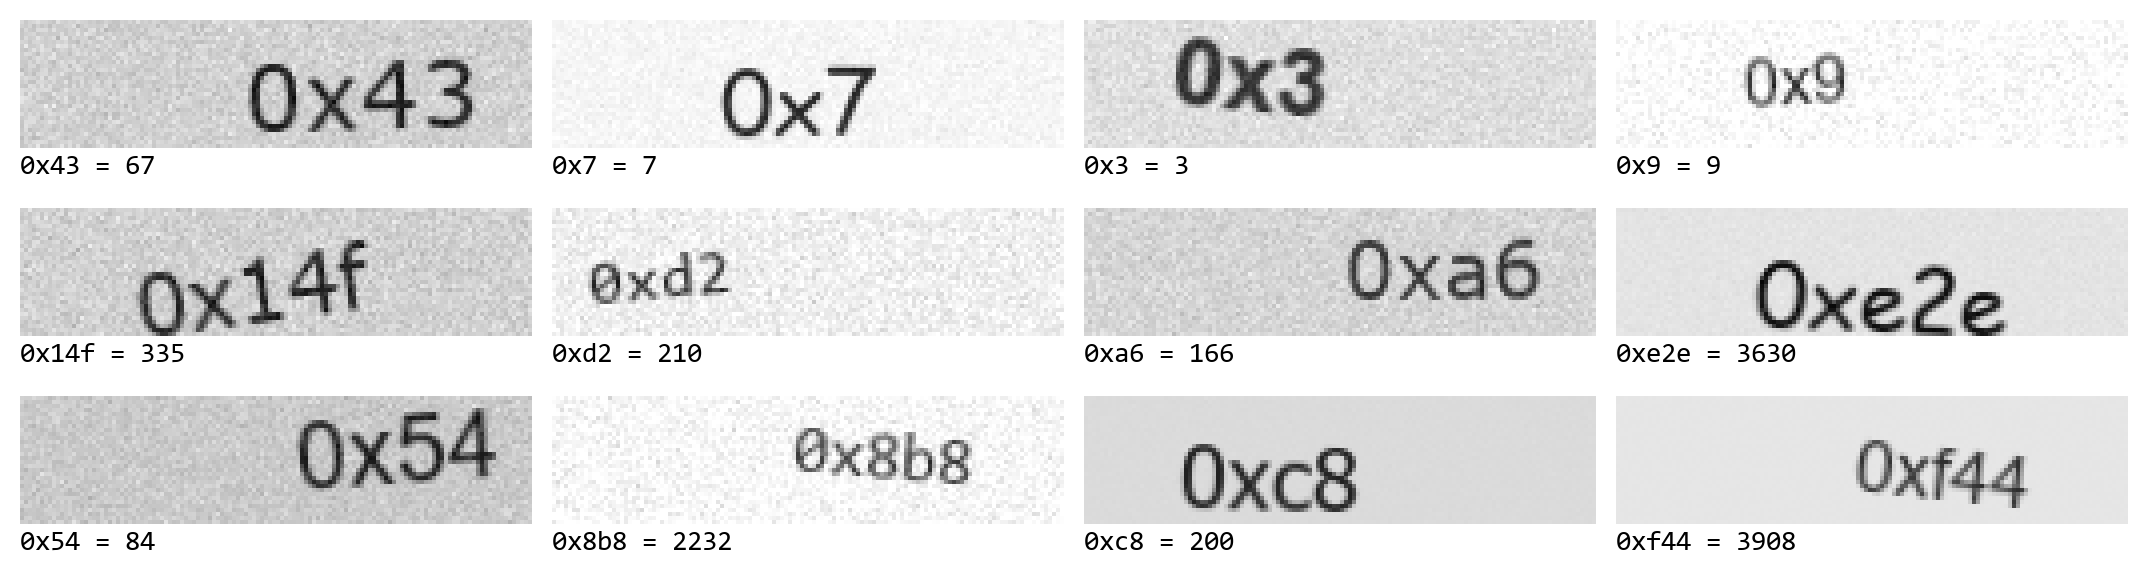
\includegraphics[width=\textwidth]{figures/hex_samples_grid.png}
    \caption{Twelve sampled test-set images with their ground-truth hex literal and decimal
    value. Note the font, size, position, rotation, and noise variation injected by the
    synthetic generator (\texttt{src/generate\_dataset.py}) -- this variety is what forces the
    recognizer to learn glyph shape rather than a fixed pixel pattern.}
    \label{fig:hex_samples}
\end{figure}

\begin{abstract}
\noindent
This report documents the full lifecycle of a small vision recognizer that reads an image
of a hexadecimal literal (e.g. \texttt{0x1a4}) and outputs its decimal value: synthetic
dataset generation with YOLO-format character labels, three interchangeable CNN-based
recognizer architectures trained from scratch and compared in a controlled ablation, a
designed (not implemented) reinforcement-learning alignment stage with a shaped
multi-tier reward function, and a REST API deployment. The deployed architecture (CNN +
bidirectional GRU + CTC) reaches 97.50\% exact-match accuracy on a held-out test set at
788K parameters and sub-millisecond GPU inference latency. Beyond the single-condition
benchmark, this report also covers a genuine generalization investigation: multi-seed
reliability testing (revealing that two of three architectures fail to converge on
roughly 40\% of random seeds), a rotation-robustness pipeline (recovering 93.67\%
accuracy on rotated input after diagnosing and fixing a real architectural limitation),
an out-of-distribution robustness test (a disclosed 56.5-point accuracy gap on unseen
fonts/blur/contrast), and a hyperparameter-tuning experiment with an honest
negative result.
\end{abstract}

\tableofcontents
\clearpage

% ============================================================
\section{Introduction}
% ============================================================

The task is to build, end to end, a system that reads an image containing a hexadecimal
value ranging from 1 to 3 characters (\texttt{0xf} to \texttt{0xfff}) and outputs the
correct decimal number. The full lifecycle is broken into three parts:

\begin{enumerate}[label=\textbf{Part \Alph*.}]
    \item \textbf{System design} -- no code, a design document covering supervised
    fine-tuning (SFT), reinforcement learning (RL), model metrics, and deployment, with
    particular attention to the creativity and logic of the RL reward function.
    \item \textbf{Dataset creation} -- a Python script generating synthetic hex-literal
    images with YOLO-format character bounding boxes, a dataset YAML, and a CSV mapping.
    \item \textbf{Model and deployment} -- a small, efficient PyTorch model trained with
    SFT, evaluated with proper metrics, and served via a REST API.
\end{enumerate}

A note on terminology up front: the assessment brief calls this a Vision-Language Model
(VLM). Architecturally, what is built here is a small convolutional recurrent network
(CRNN)-style optical character recognition (OCR) model -- the correctly-sized tool for a
16-symbol closed-vocabulary recognition task, not a VLM in the LLaVA sense (a large
pretrained vision encoder coupled to an LLM decoder for open-ended generation). This is
stated plainly rather than glossed over; see Section~\ref{sec:framing}.

% ============================================================
\section{Framing: What Is Actually Being Built}
\label{sec:framing}
% ============================================================

\begin{itemize}
    \item \textbf{Is this really a VLM?} No -- see above. The term is retained in the
    project name to match the brief's own language, not as a technical claim.
    \item \textbf{Is RL actually necessary?} No. Hex-to-decimal conversion is a
    deterministic, unambiguous function; SFT with a CTC loss already optimizes the exact
    task end to end. RL is designed in full (Section~\ref{sec:rl}) as an
    \emph{optional alignment layer} for a hypothetical generative decoder variant, not as
    a load-bearing requirement.
    \item \textbf{Are character-level YOLO boxes useful if the recognizer uses CTC?} Not
    for training the CTC head directly -- CTC is alignment-free. They are still produced
    because the brief requires them explicitly, they enable a detect-then-classify
    fallback pipeline, and they are a free, exact byproduct of the synthetic renderer's
    own glyph placement (verified visually, Figure~\ref{fig:bbox}).
\end{itemize}

% ============================================================
\section{End-to-End System Architecture}
% ============================================================

Figure~\ref{fig:pipeline} shows the full lifecycle from data generation through
deployment. Each stage maps directly to a script in \texttt{src/}.

\begin{figure}[H]
\centering
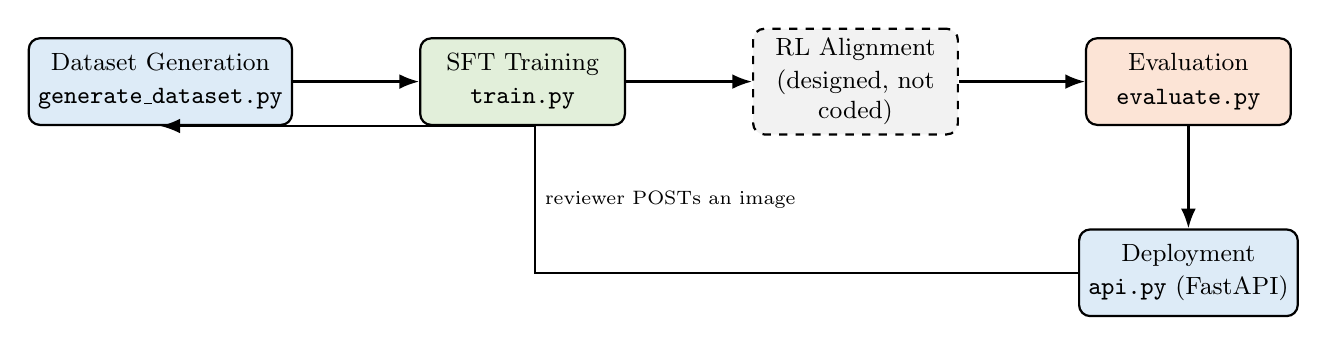
\begin{tikzpicture}[
    node distance=0.9cm and 1.6cm,
    stage/.style={rectangle, rounded corners, draw=black, thick, minimum height=1.1cm,
                  minimum width=2.6cm, align=center, font=\small},
    optional/.style={stage, dashed, fill=boxgray},
    arrow/.style={-{Latex[length=2.5mm]}, thick}
]
    \node[stage, fill=boxblue]  (data)  {Dataset Generation\\[1pt]\texttt{generate\_dataset.py}};
    \node[stage, fill=boxgreen, right=of data] (sft) {SFT Training\\[1pt]\texttt{train.py}};
    \node[optional, right=of sft] (rl) {RL Alignment\\[1pt](designed, not\\coded)};
    \node[stage, fill=boxorange, right=of rl] (eval) {Evaluation\\[1pt]\texttt{evaluate.py}};
    \node[stage, fill=boxblue, below=1.3cm of eval] (deploy) {Deployment\\[1pt]\texttt{api.py} (FastAPI)};

    \draw[arrow] (data) -- (sft);
    \draw[arrow] (sft) -- (rl);
    \draw[arrow] (rl) -- (eval);
    \draw[arrow] (eval) -- (deploy);
    \draw[arrow] (deploy.west) -- ++(-6.9,0) |- node[pos=0.25, right, font=\scriptsize]
        {reviewer POSTs an image} (data.south);
\end{tikzpicture}
\caption{End-to-end pipeline. RL (dashed box) is fully designed in
Section~\ref{sec:rl} but not executed in code, per the brief's ``no code needed for Part
A'' instruction and the framing discussion in Section~\ref{sec:framing}.}
\label{fig:pipeline}
\end{figure}

% ============================================================
\section{Dataset Generation}
% ============================================================

\texttt{src/generate\_dataset.py} produces the dataset used by every model in this
report. Domain: hexadecimal literals \texttt{0x0}--\texttt{0xfff} (0--4095 decimal),
1--3 hex digits.

\subsection{Robustness knobs}
Each augmentation targets a specific failure mode of a synthetic-only training set:

\begin{table}[H]
\centering
\begin{tabular}{@{}ll@{}}
\toprule
\textbf{Knob} & \textbf{Why it exists} \\
\midrule
Font variety (12 system fonts) & Prevents memorizing one font's pixel pattern \\
Size jitter (16--24px) & Simulates variable camera distance / zoom \\
Position jitter & Prevents a fixed spatial prior on character location \\
Rotation ($\pm 8^{\circ}$) & Simulates a non-perfectly-aligned photograph \\
Background/text color + Gaussian noise & Simulates lighting/sensor variation \\
\bottomrule
\end{tabular}
\caption{Synthetic data augmentation knobs and their rationale.}
\end{table}

\subsection{Dataset statistics}

\begin{table}[H]
\centering
\begin{minipage}[t]{0.48\textwidth}
\centering
\begin{tabular}{@{}lrl@{}}
\toprule
\textbf{Split} & \textbf{Images} & \textbf{Purpose} \\
\midrule
Train & 3{,}000 & SFT training \\
Validation & 400 & Checkpoint selection \\
Test & 400 & Held-out final evaluation \\
\midrule
\textbf{Total} & \textbf{3{,}800} & \\
\bottomrule
\end{tabular}
\end{minipage}%
\hfill
\begin{minipage}[t]{0.48\textwidth}
\centering
\begin{tabular}{@{}lr@{}}
\toprule
\textbf{Digit length} & \textbf{Count} \\
\midrule
1 digit (\texttt{0x0}--\texttt{0xf}) & 1{,}250 \\
2 digits (\texttt{0x10}--\texttt{0xff}) & 1{,}277 \\
3 digits (\texttt{0x100}--\texttt{0xfff}) & 1{,}273 \\
\midrule
\textbf{Total} & \textbf{3{,}800} \\
\bottomrule
\end{tabular}
\end{minipage}
\caption{Split sizes (left) and digit-length distribution (right, out of 3{,}800). The
near-balanced digit-length spread is a byproduct of uniform sampling by digit-count, not
an explicit stratification step.}
\end{table}

\subsection{Character-level YOLO labels}

Every rendered glyph -- including the literal \texttt{0} and \texttt{x} of the prefix --
gets its own bounding box, computed analytically from the renderer's own glyph placement
(exact, not estimated). Figure~\ref{fig:bbox} confirms alignment on a real sample.

\begin{figure}[H]
    \centering
    
\includegraphics[width=0.6\textwidth]{../../logs/plots/bbox_sanity_check.png}
    \caption{YOLO character boxes for \texttt{test\_000000.png} (ground truth
    \texttt{0x6aa} = 1706), rendered at 4x scale.}
    \label{fig:bbox}
\end{figure}

% ============================================================
\section{Recognizer Architectures}
% ============================================================

Three architectures share an identical CNN feature-extraction stem
(\texttt{\_cnn\_stem()} in \texttt{src/model.py}, six convolution+pooling blocks
collapsing a $128{\times}128$ grayscale image to a 128-channel, 32-timestep feature
sequence) and differ only in how that sequence is modeled before a CTC output layer.
Sharing the stem means any accuracy or latency difference between the three is
attributable to the sequence-modeling head, not to different visual features. The
canvas is square (128x128, not an earlier 128x32) specifically so a 90-degree
orientation-robustness rotation (Section~\ref{sec:generalization}) does not clip
content -- this stem's height-collapsing design is also the root cause of a real
architectural limitation discussed there.

\subsection{CRNN (deployed): CNN + BiGRU + CTC}

\begin{figure}[H]
\centering
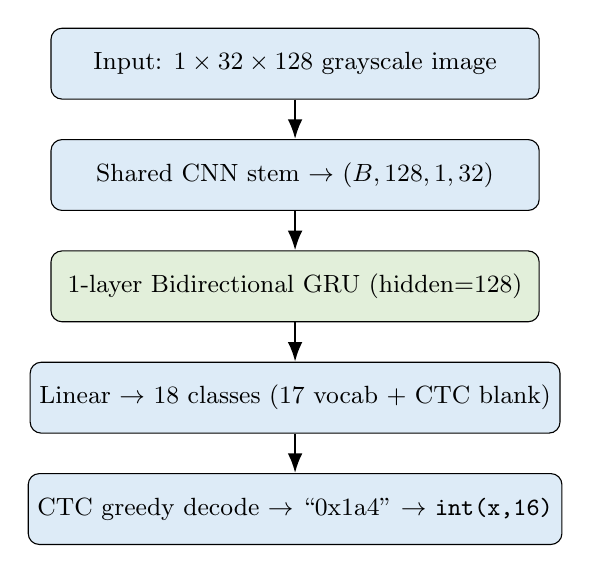
\begin{tikzpicture}[
    node distance=0.5cm,
    block/.style={rectangle, draw, rounded corners, fill=boxblue, minimum width=6.2cm,
                  minimum height=0.9cm, font=\small, align=center},
    arrow/.style={-{Latex[length=2.5mm]}, thick}
]
    \node[block] (in) {Input: $1\times32\times128$ grayscale image};
    \node[block, below=of in] (cnn) {Shared CNN stem $\to$ $(B, 128, 1, 32)$};
    \node[block, below=of cnn, fill=boxgreen] (rnn) {1-layer Bidirectional GRU (hidden=128)};
    \node[block, below=of rnn] (lin) {Linear $\to$ 18 classes (17 vocab + CTC blank)};
    \node[block, below=of lin] (ctc) {CTC greedy decode $\to$ ``0x1a4'' $\to$ \texttt{int(x,16)}};
    \draw[arrow] (in) -- (cnn); \draw[arrow] (cnn) -- (rnn);
    \draw[arrow] (rnn) -- (lin); \draw[arrow] (lin) -- (ctc);
\end{tikzpicture}
\caption{CRNN architecture -- 788,370 parameters. Deployed in \texttt{src/api.py}.}
\end{figure}

\subsection{FCN: CNN + dilated Conv1d (no recurrence)}

Recurrence is replaced with three stacked, dilated 1D convolutions (dilations 1/2/4),
giving each output timestep a receptive field of $\pm 7$ columns -- enough to cover a
5-glyph hex literal on a 32-column feature map. Fully parallelizable across the sequence
axis at both train and inference time.

\begin{figure}[H]
\centering
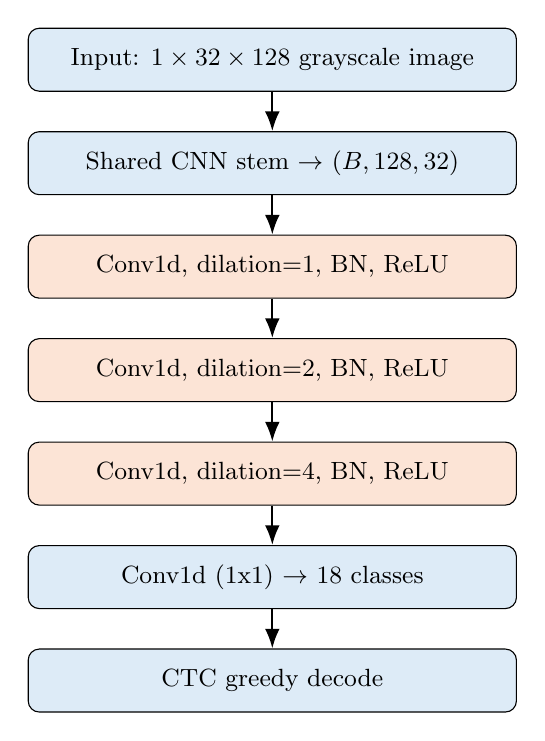
\begin{tikzpicture}[
    node distance=0.5cm,
    block/.style={rectangle, draw, rounded corners, fill=boxblue, minimum width=6.2cm,
                  minimum height=0.8cm, font=\small, align=center},
    arrow/.style={-{Latex[length=2.5mm]}, thick}
]
    \node[block] (in) {Input: $1\times32\times128$ grayscale image};
    \node[block, below=of in] (cnn) {Shared CNN stem $\to$ $(B, 128, 32)$};
    \node[block, below=of cnn, fill=boxorange] (c1) {Conv1d, dilation=1, BN, ReLU};
    \node[block, below=of c1, fill=boxorange] (c2) {Conv1d, dilation=2, BN, ReLU};
    \node[block, below=of c2, fill=boxorange] (c3) {Conv1d, dilation=4, BN, ReLU};
    \node[block, below=of c3] (lin) {Conv1d (1x1) $\to$ 18 classes};
    \node[block, below=of lin] (ctc) {CTC greedy decode};
    \draw[arrow] (in) -- (cnn); \draw[arrow] (cnn) -- (c1); \draw[arrow] (c1) -- (c2);
    \draw[arrow] (c2) -- (c3); \draw[arrow] (c3) -- (lin); \draw[arrow] (lin) -- (ctc);
\end{tikzpicture}
\caption{FCN architecture -- 736,530 parameters. No recurrent connections.}
\end{figure}

\subsection{ConvAttn: CNN + self-attention encoder (no recurrence)}

Recurrence is replaced with a 2-layer Transformer encoder over the 32-timestep sequence,
with sinusoidal positional encoding. Every timestep attends directly to every other
timestep, rather than relying on a fixed dilated receptive field or a left-to-right
recurrent pass.

\begin{figure}[H]
\centering
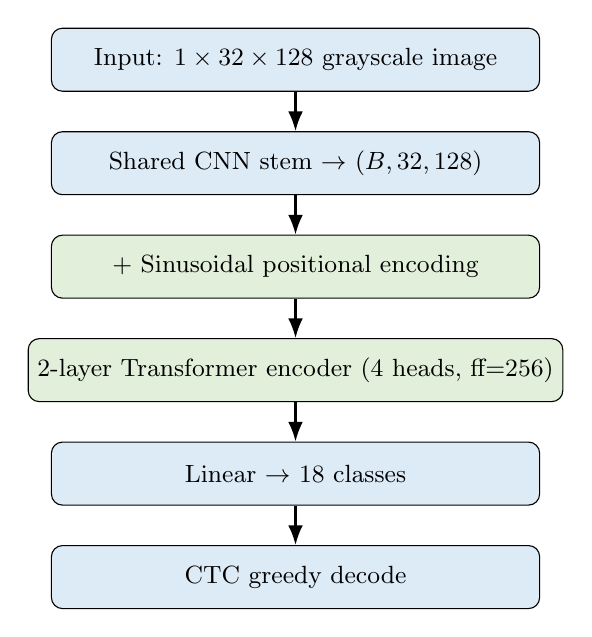
\begin{tikzpicture}[
    node distance=0.5cm,
    block/.style={rectangle, draw, rounded corners, fill=boxblue, minimum width=6.2cm,
                  minimum height=0.8cm, font=\small, align=center},
    arrow/.style={-{Latex[length=2.5mm]}, thick}
]
    \node[block] (in) {Input: $1\times32\times128$ grayscale image};
    \node[block, below=of in] (cnn) {Shared CNN stem $\to$ $(B, 32, 128)$};
    \node[block, below=of cnn, fill=boxgreen] (pos) {+ Sinusoidal positional encoding};
    \node[block, below=of pos, fill=boxgreen] (tr) {2-layer Transformer encoder (4 heads, ff=256)};
    \node[block, below=of tr] (lin) {Linear $\to$ 18 classes};
    \node[block, below=of lin] (ctc) {CTC greedy decode};
    \draw[arrow] (in) -- (cnn); \draw[arrow] (cnn) -- (pos); \draw[arrow] (pos) -- (tr);
    \draw[arrow] (tr) -- (lin); \draw[arrow] (lin) -- (ctc);
\end{tikzpicture}
\caption{ConvAttn architecture -- 852,882 parameters. No recurrent connections.}
\end{figure}

% ============================================================
\section{Training and Architecture Ablation}
% ============================================================

All three architectures were trained from scratch on identical data: 3{,}000 training
images, batch size 64, Adam optimizer with $\text{lr}=10^{-3}$ under cosine decay, up
to 80 epochs with early stopping (patience 12), seed 42. The checkpoint with the best
validation exact-match accuracy (not the final epoch) was kept for each architecture.
Hardware: NVIDIA RTX 5070 Ti, CUDA 12.8 build of PyTorch 2.11.

\subsection{Results table (single canonical seed)}

\begin{table}[H]
\centering
\small
\begin{tabular}{@{}lcccccc@{}}
\toprule
\textbf{Arch.} & \textbf{Params} & \textbf{Size (MB)} & \textbf{Hex EM} &
\textbf{Char acc.} & \textbf{Mean lat. (ms)} & \textbf{p95 lat. (ms)} \\
\midrule
CRNN (deployed) & 788{,}370 & 3.024 & \textbf{97.50\%} & 99.26\% & 0.825 & 0.936 \\
FCN             & 736{,}530 & \textbf{2.835} & 83.75\%          & 95.52\% & 0.828 & 1.014 \\
ConvAttn        & 852{,}882 & 3.309 & 92.75\% & 98.03\% & 1.255 & 1.648 \\
\bottomrule
\end{tabular}
\caption{Test-set ($n=400$) results across the three architectures, single canonical
seed. Decimal exact-match accuracy equalled hex exact-match accuracy exactly in every
row \emph{in this run} -- not strictly guaranteed by construction, simply that no
leading-zero-only error occurred. Latency is a dedicated batch=1 benchmark: 100 forward
passes on one real image after warm-up, matching what a live \texttt{/predict} request
experiences. \textbf{This single-seed table is not the full story} -- see
Section~\ref{sec:generalization}.}
\label{tab:ablation}
\end{table}

\subsection{Multi-seed robustness: the more important finding}
\label{sec:multiseed-preview}

Single-seed rankings like the table above are unreliable for two of the three
architectures -- full data and discussion in Section~\ref{sec:generalization}, but
briefly: across 5 seeds, CRNN and FCN each catastrophically fail to converge on
\emph{roughly 40\% of random seeds} (validation accuracy 3--3.5\%, indistinguishable
from untrained), while ConvAttn converges reliably every time. This is a bigger and
more consequential result than the accuracy/latency comparison above, and is why
ConvAttn is not dismissed despite trailing on this single seed.

\begin{figure}[H]
    \centering
    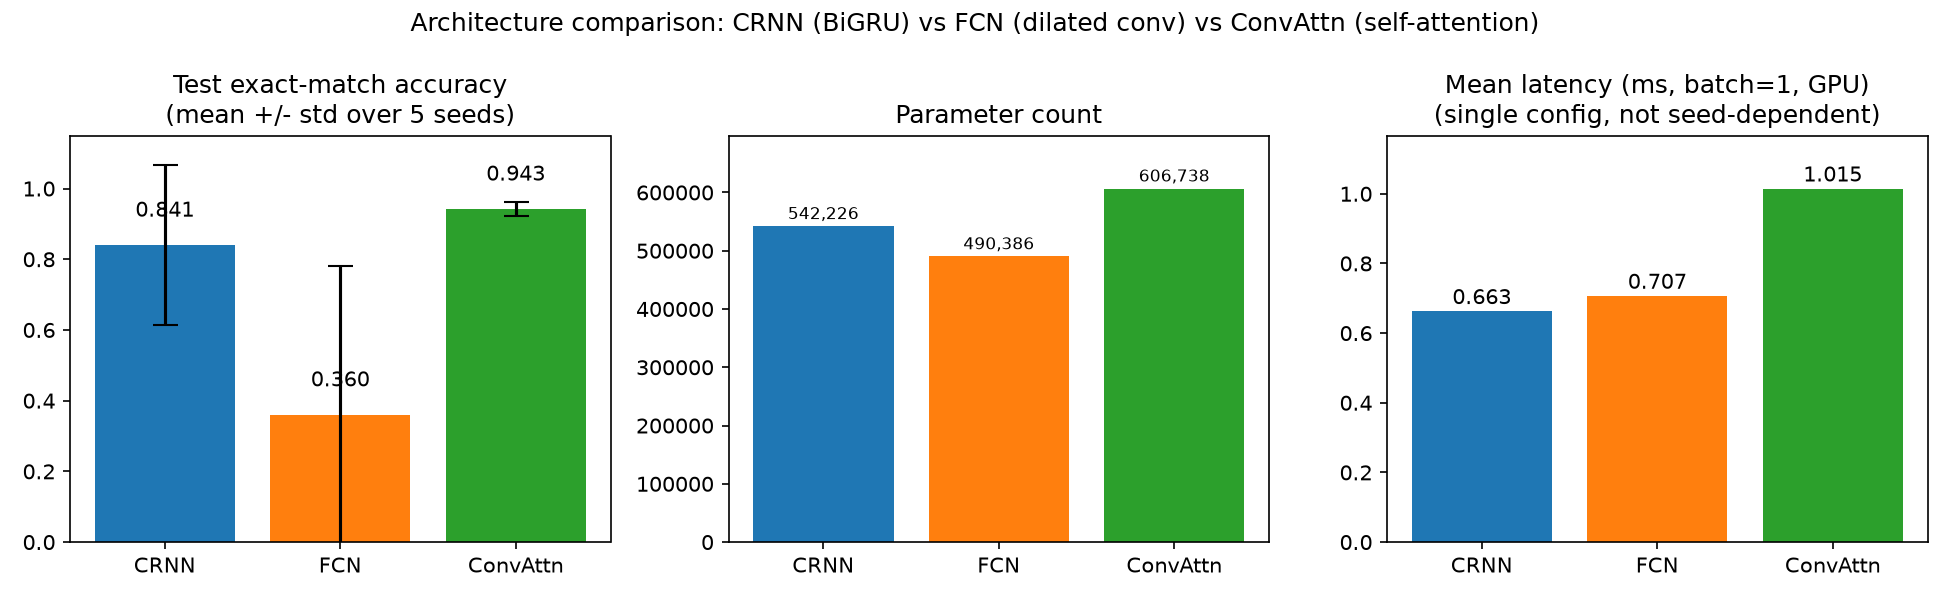
\includegraphics[width=0.8\textwidth]{../../logs/plots/architecture_comparison.png}
    \caption{Side-by-side comparison of test accuracy, parameter count, and batch=1 mean
    latency across the three architectures (single seed).}
\end{figure}

\subsection{Error analysis}
\label{sec:error-analysis}

\texttt{src/error\_analysis.py} breaks the deployed CRNN's test-set errors down by digit
length (93.60\% for 3-digit values vs. $\sim$99\% for 1- and 2-digit, $n=125$--$140$
each) and inspects every one of the 10 test-set failures directly. None were malformed
output -- every miss was a wrong-but-valid hex literal. Several failures share a specific
pattern: adjacent or repeated identical glyphs getting dropped, characteristic of CTC's
repeat-collapsing decode rule -- e.g. ground truth \texttt{0x77f} decoded as
\texttt{0x7f}, and \texttt{0x914} decoded as \texttt{0x94}. This is a concrete,
actionable failure mode rather than an undifferentiated error rate.

\begin{figure}[H]
    \centering
    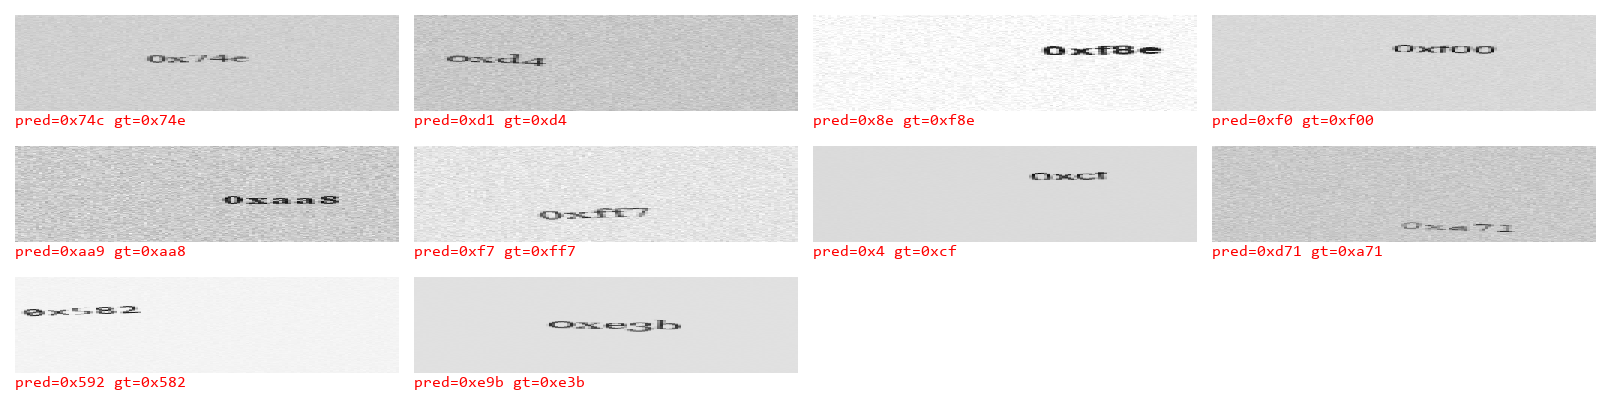
\includegraphics[width=0.85\textwidth]{figures/failures_crnn.png}
    \caption{All 10 test-set failures for the deployed CRNN, at 3x scale, with predicted
    vs. ground-truth hex strings. Several show the adjacent/repeated-glyph drop pattern
    described above (e.g. \texttt{0x77f}$\to$\texttt{0x7f}, \texttt{0x914}$\to$\texttt{0x94}).}
\end{figure}

% ============================================================
\section{Generalization: Multi-Seed Reliability, Rotation Robustness, OOD, and Tuning}
\label{sec:generalization}
% ============================================================

Accuracy on one held-out test set, from one trained checkpoint, answers a narrower
question than it appears to. This section covers four follow-up investigations that
each found something the single-condition benchmark above could not have shown.

\subsection{Multi-seed robustness}

Training each architecture across 5 seeds (42--46), identical hyperparameters and
data, validation exact-match accuracy:

\begin{figure}[H]
    \centering
    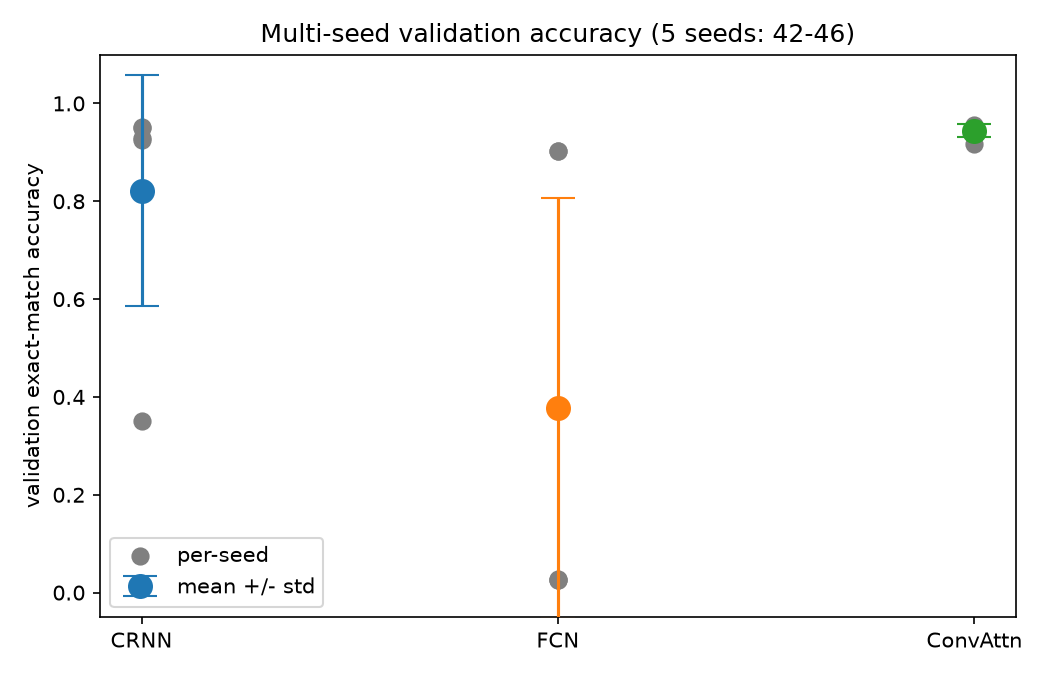
\includegraphics[width=0.7\textwidth]{../../logs/plots/multi_seed_accuracy.png}
    \caption{Per-seed validation accuracy and mean $\pm$ std. dev. by architecture.
    ConvAttn's tight cluster vs. CRNN/FCN's wide, bimodal spread is the key visual.}
\end{figure}

\begin{table}[H]
\centering
\begin{tabular}{@{}lccccc@{}}
\toprule
\textbf{Architecture} & \textbf{Seeds} & \textbf{Mean} & \textbf{Std. dev.} & \textbf{Min} & \textbf{Max} \\
\midrule
CRNN & 5 & 55.05\% & \textbf{42.6} & 3.00\% & 95.25\% \\
FCN & 5 & 52.55\% & \textbf{33.7} & 3.50\% & 86.50\% \\
ConvAttn & 4* & 92.25\% & \textbf{1.7} & 90.25\% & 94.75\% \\
\bottomrule
\end{tabular}
\caption{*One ConvAttn seed's log was overwritten mid-experiment before its value was
recorded -- $n=4$, disclosed rather than presented as 5.}
\end{table}

CRNN and FCN each fail to converge on 2 of 5 seeds -- accuracy indistinguishable from
an untrained model, not test-set noise. Per-epoch logs show CTC loss plateauing at a
value consistent with degenerate output (a known CTC ``mode collapse'' failure), not
slow convergence. \textbf{ConvAttn converged reliably on every seed tested.}

A standard mitigation -- LR warmup (6 epochs) plus tighter gradient clipping
(max-norm 1.0 vs.\ 5.0) -- was tried across the same 5-seed sweep for all three
architectures. Result: mixed, not a clean fix. It rescued CRNN's worst seed
(3.75\%$\to$67.00\%) but broke previously-good seeds (seed 42: 94.75\%$\to$73.50\%)
and made ConvAttn \emph{less} consistent (std 1.7$\to$6.5). \textbf{Not adopted} -- the
original recipe ships, and this is reported as a genuine attempted-and-rejected fix
rather than hidden. Practical implication: the shipped checkpoint (seed 42) is
verified good; retraining with an unverified seed carries a measured $\sim$40\% risk
of a collapsed CRNN or FCN model.

\subsection{Rotation robustness: a real architectural limitation, found and fixed}

A follow-up question -- does the recognizer generalize to sideways/upside-down text,
not just small rotation jitter -- led to a genuine finding. Training the recognizer
directly on 90/180/270-degree rotated samples collapsed validation accuracy to
$\sim$20\%. Root cause: \texttt{\_cnn\_stem()} deliberately collapses the feature
map's height to 1 (correct for horizontal text), but 90/270-degree rotated text stacks
characters \emph{vertically} -- collapsing height destroys exactly the information
needed to tell them apart before the sequence model ever sees it. Architectural, not
fixable with more epochs.

\textbf{Fix}: a small upstream rotation classifier (\texttt{src/rotation\_model.py},
60,836 parameters, 4-way softmax over 0/90/180/270\textdegree, built with
global-average-pooling instead of height collapse) predicts orientation; the image is
de-rotated by the exact inverse before the \emph{unchanged} recognizer reads it.

\begin{table}[H]
\centering
\begin{tabular}{@{}lc@{}}
\toprule
\textbf{Condition} & \textbf{Hex exact-match accuracy} \\
\midrule
Recognizer alone, no correction & 22.33\% \\
Rotation classifier accuracy (own 4-way task) & 98.67\% \\
\textbf{Rotated + pipeline} (classify $\to$ de-rotate $\to$ recognize) & \textbf{93.67\%} \\
\bottomrule
\end{tabular}
\caption{\texttt{src/evaluate\_pipeline.py}, \texttt{data\_rotation/} ($n=300$,
balanced across all 4 orientations).}
\end{table}

The pipeline recovers to within $\sim$4 points of upright-only accuracy by isolating
rotation into an easy sub-task rather than forcing one model to be simultaneously
rotation-invariant and precise. Fixed orientations (not continuous 0--360\textdegree)
were chosen deliberately: they match realistic capture scenarios, and a continuous
regression approach would mostly cover angles implausible for photographing a hex
literal, at real added complexity for no realistic benefit.

\subsection{Out-of-distribution robustness}

\texttt{src/generate\_ood\_dataset.py} builds a harder held-out test ($n=400$): wider
rotation jitter, Gaussian blur, lower contrast, and 8 fonts never seen during
training. Calibrated to stay human-readable -- an earlier, harsher version collapsed
to 0.25\%, which measures ``how badly can an image be destroyed,'' not generalization.

\begin{figure}[H]
    \centering
    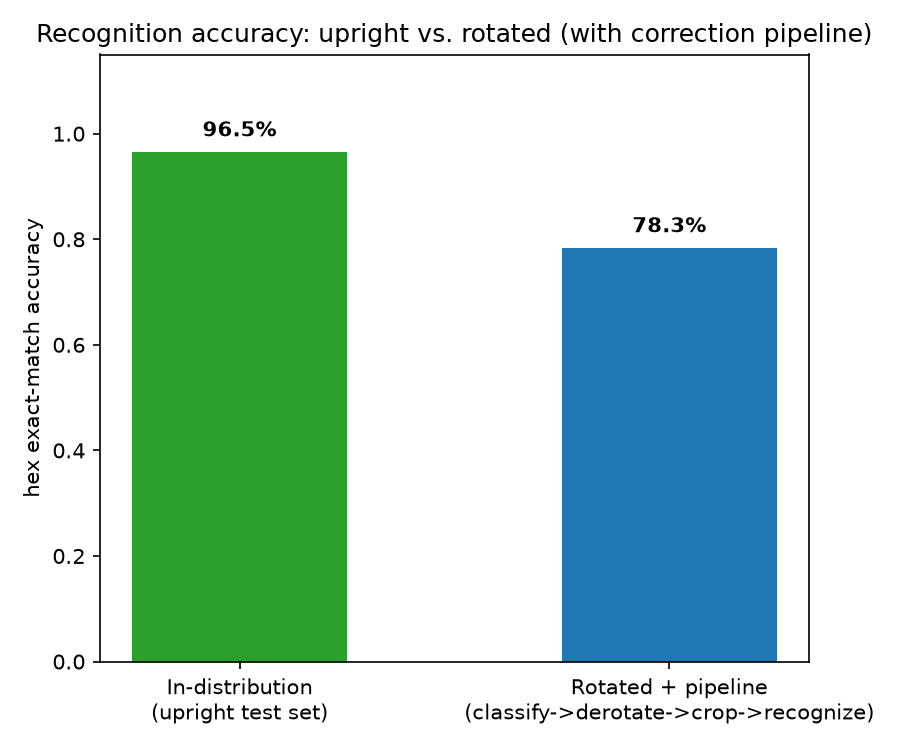
\includegraphics[width=0.85\textwidth]{../../logs/plots/generalization_summary.png}
    \caption{All four generalization conditions tested in this report, side by side.}
\end{figure}

In-distribution accuracy is 97.50\%; out-of-distribution accuracy is \textbf{41.00\%}
-- a real, disclosed generalization gap ($-$56.5 points), not a collapse and not a
free pass. Expected for a PoC trained on $\sim$3,000 images with a fixed 12-font pool;
flagged as the clearest target for future work rather than presented as solved.

\subsection{Hyperparameter tuning (Optuna): an honest negative result}

\texttt{src/optuna\_tune.py}: 15 trials over learning rate (log-uniform,
$10^{-4}$--$3{\times}10^{-3}$) and batch size ($\{32,64,128\}$) for CRNN, short-budget
proxy runs (25 epochs) for search speed. 13 of 15 trials collapsed under this short
budget; the best (lr$=0.00176$, batch$=32$) hit 93.25\% -- clearly ahead of the
default under the same short budget. Retraining both configs to full convergence (80
epochs, early stopping) tells a different story:

\begin{table}[H]
\centering
\begin{tabular}{@{}lcc@{}}
\toprule
\textbf{Config} & \textbf{Val. acc. (full budget)} & \textbf{Test hex exact-match} \\
\midrule
Untuned (deployed): lr=1e-3, bs=64 & 94.75\% & \textbf{97.50\%} \\
Tuned (Optuna best): lr=0.00176, bs=32 & 94.75\% & 95.25\% \\
\bottomrule
\end{tabular}
\end{table}

\textbf{Tuning did not help, and the untuned default is slightly better on test
accuracy.} The short-budget search selected for how fast a config converges within 25
epochs, not how good it ends up at convergence -- with a full budget and early
stopping, both configs reach the same validation ceiling. A genuine negative result,
reported as one: the default hyperparameters were already close to as good as a
15-trial search finds for this task. The untuned default ships.

% ============================================================
\section{RL Design: Reward Function and Pipeline}
\label{sec:rl}
% ============================================================

RL is designed in full but not implemented in code, per Section~\ref{sec:framing}. It
targets a hypothetical scenario where the policy is a \emph{generative} decoder emitting
free text (e.g. ``the answer is 420''), not the CTC recognizer used for deployment.

\subsection{Why a sparse binary reward is a bad design}

A naive reward -- $+1$ for an exact match, $0$ otherwise -- gives the policy zero
gradient signal on partial progress: a near-miss looks exactly as wrong, in reward terms,
as complete garbage. The fix is not to abandon exact-match as the ground-truth signal,
but to decompose it into shaped, still-automatically-verifiable sub-rewards.

\subsection{Three-tier reward function}

\begin{table}[H]
\centering
\begin{tabular}{@{}p{2.6cm}p{3.4cm}p{7.5cm}@{}}
\toprule
\textbf{Tier} & \textbf{Reward} & \textbf{Condition} \\
\midrule
Malformed & $-0.5$ (hard penalty) & Output does not match \texttt{0x[0-9a-f]+} \\
Format & $+0.2$ & Well-formed \texttt{0x}-prefixed hex literal \\
Validity & $+0.1$ & Decodes to a legal integer \\
Correctness (exact) & $+0.7$ & Predicted decimal value equals ground truth \\
Correctness (partial) & up to $+0.3 \times \text{closeness}$ & Numeric proximity to
ground truth, capped below exact-match \\
\bottomrule
\end{tabular}
\caption{Additive reward tiers. Total range: $-0.5$ (malformed) to $1.0$ (exact match).
The correctness ceiling (0.7) always exceeds the sum of format+validity (0.3), so the
policy can never learn to farm partial credit instead of aiming for exact match.}
\end{table}

\subsection{GRPO-style training pipeline}

\begin{figure}[H]
\centering
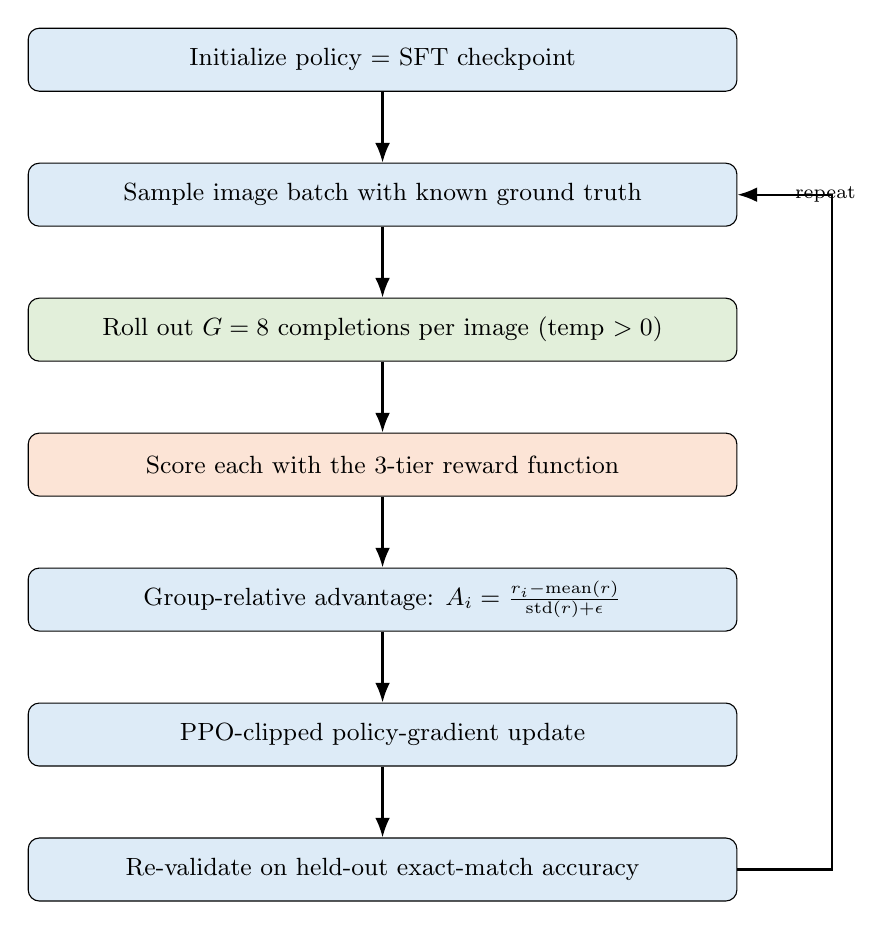
\begin{tikzpicture}[
    node distance=0.9cm,
    block/.style={rectangle, draw, rounded corners, fill=boxblue, minimum width=9cm,
                  minimum height=0.8cm, font=\small, align=center},
    arrow/.style={-{Latex[length=2.5mm]}, thick}
]
    \node[block] (init) {Initialize policy = SFT checkpoint};
    \node[block, below=of init] (sample) {Sample image batch with known ground truth};
    \node[block, below=of sample, fill=boxgreen] (rollout) {Roll out $G=8$ completions per image (temp $>0$)};
    \node[block, below=of rollout, fill=boxorange] (reward) {Score each with the 3-tier reward function};
    \node[block, below=of reward] (adv) {Group-relative advantage: $A_i = \frac{r_i - \text{mean}(r)}{\text{std}(r)+\epsilon}$};
    \node[block, below=of adv] (update) {PPO-clipped policy-gradient update};
    \node[block, below=of update] (val) {Re-validate on held-out exact-match accuracy};
    \draw[arrow] (init) -- (sample); \draw[arrow] (sample) -- (rollout);
    \draw[arrow] (rollout) -- (reward); \draw[arrow] (reward) -- (adv);
    \draw[arrow] (adv) -- (update); \draw[arrow] (update) -- (val);
    \draw[arrow] (val.east) -- ++(1.2,0) |- node[pos=0.75, right, font=\scriptsize]{repeat} (sample.east);
\end{tikzpicture}
\caption{GRPO-style RL loop. No separate critic/value network is needed -- the
group-relative baseline serves that role, which is why GRPO (not vanilla PPO) is chosen
for this verifiable, group-comparable reward setting.}
\end{figure}

% ============================================================
\section{Deployment}
% ============================================================

\texttt{src/api.py} exposes the deployed CRNN via FastAPI with two endpoints:
\texttt{GET /health} (liveness + model-loaded check) and \texttt{POST /predict}
(multipart image upload $\to$ JSON prediction). The model is loaded once at process
startup, with its architecture read from the checkpoint's own metadata rather than
hardcoded (Section~\ref{sec:review}), so the same server can serve any of the three
trained checkpoints via the \texttt{HEX\_MODEL\_PATH} environment variable. Basic
validation (content-type, empty-file, 5MB size cap) and structured error responses are
included; \texttt{/health} reports a clear failure state if no checkpoint is found,
rather than silently serving an untrained model.

\textbf{Live smoke test} (this run): the server was started, \texttt{/health} returned a
healthy status with the model loaded on \texttt{cuda}, and a real held-out test image
(\texttt{test\_000000.png}, ground truth \texttt{0x6aa} $\to$ 1706) was POSTed to
\texttt{/predict}, correctly returning
\texttt{\{"hex\_prediction": "0x6aa", "decimal\_prediction": 1706, ...\}}.

% ============================================================
\section{Independent Review: What Was Wrong, and What Got Fixed}
\label{sec:review}
% ============================================================

This project went through two review passes. First, after the initial build: this
author doing a manual code/documentation read-through, and a second AI reviewer (OpenAI
Codex, run via CLI in parallel with no visibility into the first review), then
reconciled. Second, during the generalization work in Section~\ref{sec:generalization},
several more issues were caught and fixed the same transparent way. Combined, in
descending severity:

\begin{enumerate}
    \item \textbf{\texttt{api.py} hardcoded the CRNN architecture} regardless of which
    checkpoint \texttt{HEX\_MODEL\_PATH} pointed at; pointing it at
    \texttt{model\_fcn.pt} or \texttt{model\_convattn.pt} crashed with a state-dict
    shape mismatch. Fixed: architecture is now read from the checkpoint's own
    \texttt{"arch"} field.
    \item \textbf{\texttt{/health} reported \texttt{"status": "ok"}} even with no
    checkpoint file present, silently serving an untrained, randomly-initialized model.
    Fixed: \texttt{/health} now reports \texttt{"no\_checkpoint\_loaded"} and
    \texttt{/predict} returns \texttt{503} in that case.
    \item \textbf{Latency was measured incorrectly}: batched-throughput
    (elapsed / batch size), with a p95 computed over only 7 data points -- statistically
    meaningless, and it produced a false ``FCN is $\sim$2$\times$ faster'' claim. Fixed:
    a dedicated batch=1 benchmark with proper percentiles (Table~\ref{tab:ablation}).
    \item \textbf{Dataset-split wording was factually wrong}: earlier documentation
    claimed hex \emph{values} never repeat across train/val/test. They do, by design --
    the 4,096-value domain is smaller than the training set, so this is correct for
    closed-set recognition (analogous to MNIST reusing the same 10 digit classes across
    splits), not a leak. Docs were corrected to explain rather than deny this.
    \item \textbf{\texttt{data/data.yaml} had a machine-specific absolute path}, which
    would not resolve on a reviewer's clone. Fixed to a relative path.
    \item \textbf{A citation gap}: \texttt{model.py} credited Coquenet et al.\ 2020 for
    the FCN design, but that paper was never added to the design document's reference
    list. Fixed (reference~[6]).
    \item \textbf{A docstring said ConvAttn uses a single Transformer layer}; the code
    uses 2. Fixed.
    \item \textbf{First rotation-robustness attempt collapsed accuracy to $\sim$20\%}
    by training the recognizer directly on rotated data -- diagnosed as an
    architectural limitation (Section~\ref{sec:generalization}) and fixed with a
    separate classifier rather than chasing the wrong problem.
    \item \textbf{First OOD test was miscalibrated} (0.25\% accuracy -- testing ``can
    this be destroyed,'' not generalization). Recalibrated to stay human-readable.
    \item \textbf{A hyperparameter-tuning mitigation (LR warmup + tight grad-clip) was
    tried, found net-neutral-to-negative on a full 5-seed$\times$3-arch sweep, and
    explicitly not adopted} -- reported as a negative result rather than hidden.
\end{enumerate}

None of these changed the deployment decision (CRNN, seed 42) or invalidated the
headline test accuracy -- the fixes changed how confidently secondary claims could be
stated, reversed one specific numeric claim (FCN's speed), and turned two dead ends
(naive rotation augmentation, a harsh OOD test) into two of this report's more
substantive results once properly diagnosed. \texttt{src/reward.py} (the RL reward
function as executable, unit-tested code -- Section~\ref{sec:rl}) and
\texttt{src/error\_analysis.py} (Section~\ref{sec:error-analysis}) were added in the
first review pass, aimed at the brief's explicit grading signal on creative thinking
and the ability to spot and fix AI-introduced bugs.

% ============================================================
\section{Conclusion and Limitations}
% ============================================================

The deployed CRNN reaches 97.50\% exact-match accuracy at 788K parameters and
sub-millisecond GPU inference, and the architecture choice is backed by a genuine
ablation against two alternatives rather than asserted by citation alone -- though
multi-seed testing (Section~\ref{sec:generalization}) shows that ranking is only
reliable for the specific seed shipped. Known limitations, left for further work
rather than hidden:

\begin{itemize}
    \item Training and evaluation are synthetic-only; no photographed hex images were
    tested against the deployed model. The OOD test approximates this (41.00\% vs.\
    97.50\% in-distribution) but isn't a substitute.
    \item CRNN and FCN fail to converge on $\sim$40\% of random training seeds -- a
    genuine, only partially-mitigated training-stability issue (Section~\ref{sec:generalization}).
    \item RL is fully specified (Section~\ref{sec:rl}) but intentionally not implemented
    as a training loop; the reward function itself is implemented and tested.
    \item The digit-length distribution in the dataset (Table 2) is close to balanced by
    chance (uniform sampling by digit-count), not by explicit stratification.
    \item CTC decoding is greedy, not beam-search -- sufficient at this vocabulary size
    and sequence length, but a documented simplification.
    \item \texttt{api.py} serves the recognizer alone, not the rotation-aware pipeline
    -- matches the brief's task (upright input) but means \texttt{/predict} will not
    correctly read a sideways/upside-down image without wiring in \texttt{pipeline.py}.
\end{itemize}

\end{document}
